\documentclass[german,10pt]{book}     
\usepackage{makeidx}
\usepackage{babel}            % Sprachunterstuetzung
\usepackage{amsmath}          % AMS "Grundpaket"
\usepackage{amssymb,amsfonts,amsthm,amscd} 
\usepackage{mathrsfs}
\usepackage{rotating}
\usepackage{sidecap}
\usepackage{graphicx}
\usepackage{color}
\usepackage{fancybox}
\usepackage{tikz}
\usetikzlibrary{arrows,snakes,backgrounds}
\usepackage{hyperref}
\hypersetup{colorlinks=true,
                    linkcolor=blue,
                    filecolor=magenta,
                    urlcolor=cyan,
                    pdftitle={Overleaf Example},
                    pdfpagemode=FullScreen,}
%\newcommand{\hyperref}[1]{\ref{#1}}
%
\definecolor{Gray}{gray}{0.80}
\DeclareMathSymbol{,}{\mathord}{letters}{"3B}
%
\newcounter{num}
\renewcommand{\thenum}{\arabic{num}}
\newenvironment{anmerkungen}
   {\begin{list}{(\thenum)}{%
   \usecounter{num}%
   \leftmargin0pt
   \itemindent5pt
   \topsep0pt
   \labelwidth0pt}%
   }{\end{list}}
%
\renewcommand{\arraystretch}{1.15}                % in Formeln und Tabellen   
\renewcommand{\baselinestretch}{1.15}                 % 1.15 facher
                                                      % Zeilenabst.
\newcommand{\Anmerkung}[1]{{\begin{footnotesize}#1 \end{footnotesize}}\\[0.2cm]}
\newcommand{\comment}[1]{}
\setlength{\parindent}{0em}           % Nicht einruecken am Anfang der Zeile 

\setlength{\textwidth}{15.4cm}
\setlength{\textheight}{23.0cm}
\setlength{\oddsidemargin}{1.0mm} 
\setlength{\evensidemargin}{-6.5mm}
\setlength{\topmargin}{-10mm} 
\setlength{\headheight}{0mm}
\newcommand{\identity}{{\bf 1}}
%
\newcommand{\vs}{\vspace{0.3cm}}
\newcommand{\noi}{\noindent}
\newcommand{\leer}{}

\newcommand{\engl}[1]{[\textit{#1}]}
\parindent 1.2cm
\sloppy

     \begin{document}   \setcounter{chapter}{2}  

\chapter{Philosophischer Hintergrund der SRT}   %  Kap. 3
\label{chap_Philosophie}

Betrachtet man vor dem Hintergrund der speziellen 
Relativit\"atstheorie das Modell von Lorentz, so  
wirkt die mechanische Kontraktion physikalischer Systeme
und die zeitliche Verz\"ogerung physikalischer Prozesse
bei einer Bewegung relativ zum \"Ather
eher befremdlich. Insbesondere der 
material\-un\-ab\-h\"angige, universelle Verk\"urzungsfaktor $\sqrt{1-(v/c)^2}$ 
erscheint auf den ersten Blick willk\"urlich. Man gewinnt den Eindruck, als ob
eine entsprechende universelle Wechselwirkung zwischen Materie und
\"Ather, die diesen Verk\"urzungsfaktor erkl\"art, nur in einem sehr 
komplizierten und unnat\"urlichen Modell beschrieben werden kann.

Dies ist jedoch nicht der Fall. Im Gegenteil, die
Maxwell-Theorie oder auch unser heutiges Standardmodell sind ebenfalls in 
der Lage, diesen Verk\"urzungsfaktor zu erkl\"aren. Der Unterschied
zwischen der speziellen Relativit\"atstheorie im Sinne von Einstein und der Lorentz'schen
Theorie (\"Ather, Verk\"urzungsfaktor, etc.) erweist sich nur als eine 
Frage der Interpretation. Der mathematische Formalismus ist derselbe und kein
Experiment kann zwischen den beiden Interpretationen unterscheiden. 
Die heute verbreitete Interpretation, nach der die Effekte der speziellen Relativit\"atstheorie
als Folgerung der Geometrie der Minkowski-Raumzeit gedeutet werden, hat den
Vorteil, keine unbeobachtbaren Elemente - die Entit\"at des \"Athers oder ein ausgezeichnetes
Ruhesystem - zu enthalten. Man spricht in diesem Zusammenhang auch gerne
von Ockhams Rasiermesser (Ockham's Razor): Hierbei handelt es sich um ein nach
Wilhelm von Ockham (1288-1347) benanntes Prinzip der Wissenschaftstheorie, wonach
ein Erkl\"arungsmodell m\"oglichst einfach sein sollte, bzw.\ zwischen zwei Modellen dasjenige
den Vorzug hat, das mit weniger Variablen auskommt.   

Andererseits ist es oft von Vorteil, m\"oglichst viele gleichberechtigte Perspektiven auf einen
Sachverhalt zu haben, und es gibt durchaus Situationen, in denen die Lorentz'sche Interpretation
der Relativit\"atstheorie eine intuitivere Vorstellung vermittelt als die Einstein'sche. Daher beginnt
dieser Abschnitt mit einer Beschreibung dieser Sichtweise. 

\section{Eine Kette gekoppelter Pendel}
\label{sec_Kette}

Wir betrachten zun\"achst ein einfaches mechanisches
Modell, in dem die L\"angenma\ss\-st\"abe eine Lorentz-Kontraktion
erfahren, wenn sie sich mit einer Geschwindigkeit
$v$ relativ zu dem absolut ruhenden Bezugssystem bewegen. Auch die
anderen bekannten Beziehungen aus der speziellen Relativit\"atstheorie
wie beispielsweise die Zeitdilatation werden in diesem Modell wiedergegeben.


\begin{figure}[htb]
\begin{picture}(400,100)(0,0)
\multiput(10,10)(20,0){20}{\line(0,1){80}}
\multiput(10,10)(20,0){20}{\circle*{10}}
\multiput(13.2,40)(20,0){19}{\makebox(0,0){${\scriptstyle \vee}$}}
\multiput(18.1,40)(20,0){19}{\makebox(0,0){${\scriptstyle \vee}$}}
\multiput(23.0,40)(20,0){19}{\makebox(0,0){${\scriptstyle \vee}$}}
\multiput(27.9,40)(20,0){19}{\makebox(0,0){${\scriptstyle \vee}$}}
\put(415,50){\vector(0,-1){40}}
\put(420,30){\makebox(0,0){${\scriptstyle g}$}}
\put(170,0){\makebox(0,0){${\scriptstyle i-1}$}}
\put(190,0){\makebox(0,0){${\scriptstyle i}$}}
\put(210,0){\makebox(0,0){${\scriptstyle i+1}$}}
\put(395,60){\makebox(0,0){${\scriptstyle l}$}}
\put(400,10){\makebox(0,0){${\scriptstyle m}$}}
\put(395,40){\makebox(0,0){${\scriptstyle D}$}}
\thicklines
\put(0,90){\line(1,0){400}}
\end{picture}
\caption{\label{fig_Pendel}%
Eine Kette harmonisch gekoppelter Pendel im
Schwerefeld der Erde. Die Pendel k\"onnen senkrecht
zur Darstellungsebene schwingen. Ihr Freiheitsgrad ist der
Auslenkungswinkel relativ zur Senkrechten. Die Pendelkugeln haben eine Masse $m$,
die harmonische Feder zwischen den Pendeln die Federkonstante $D$. Die L\"ange der
Pendel sei $l$ und $g$ sei die Schwerebeschleunigung der Erde.}
\end{figure}


Als physikalisches Modell stelle man sich eine Kette harmonisch gekoppelter
\index{Pendelkette}
Pendel in einem konstanten Gravitationsfeld vor. Die Pendel seien
mit einem Index $i$ durchnummeriert, wobei wir zun\"achst $i$ die
ganzen Zahlen durchlaufen lassen. Der Freiheitsgrad des $i$-ten 
Pendels ist der Winkel $\varphi_i$ relativ zur herabh\"angenden
Ruhelage. Die Wirkung dieses Modells lautet:
\[  S ~=~ \frac{1}{2} \int \! {\rm d} t \sum_i \left[   
       \left( \frac{\partial \varphi_i(t)}{\partial t} \right)^2 -
       D \left[ \varphi_{i+1}(t) -\varphi_i(t) \right]^2 +
       2 g \cos \varphi_i(t)  \right]  \;,    \]
und die zugeh\"orige Bewegungsgleichung des 
$i$-ten Pendels ist:
\begin{equation}
\label{discrete}
  \frac{\partial^2 \varphi_i(t)}{\partial t^2} -         
  D [\varphi_{i+1}(t) - 2 \varphi_i(t) + \varphi_{i-1}(t) ]
  + g \sin \varphi_i ~=~ 0 \;. 
\end{equation}             
Suchen wir nach L\"osungen, bei denen sich die Winkel benachbarter Pendel 
nicht wesentlich unterscheiden, muss $g\ll D$ gelten. 
In diesem Fall k\"onnen wir das diskrete Modell
durch ein kontinuierliches feldtheoretisches Modell mit der Wirkung
\[  S ~=~ \frac{1}{2} \int \! {\rm d} t\, {\rm d} x~ \left[   
        \left( \frac{\partial \varphi(x,t)}{\partial t} \right)^2 -
        \left( \frac{\partial \varphi(x,t)}{\partial x} \right)^2 +
        g \cos \varphi(x,t)  \right]     \]
und den Feldgleichungen 
\begin{equation}
\label{eq_cont}
  \frac{\partial^2 \varphi}{\partial t^2} -         
    \frac{\partial^2 \varphi}{\partial x^2} + g \sin \varphi ~=~ 0 
\end{equation}             
approximieren. Hier wurde $D=1$ gesetzt und der kontinuierliche
Parameter $x$, der den Ort entlang der Aufh\"angung bezeichnet,
ersetzt die Nummerierung der Pendel. Die folgenden \"Uberlegungen
gehen immer von diesem kontinuierlichen Modell aus.
Die Kennzeichnung der Raum-Zeit-Punkte $(x,t)$ bezieht sich jedoch auf 
eine feste, Newton'sche Hinter\-grunds\-raum\-zeit. Daher ist es auch
ganz instruktiv, sich die Kette gekoppelter Pendel vorzustellen,
da in diesem Fall der klare -- Newton'sche -- Charakter von \glqq Raum\grqq\ und
\glqq Zeit\grqq\ deutlicher wird.

Wir wissen, dass die Kontinuumsfeldgleichung (\ref{eq_cont}) invariant
\index{Lorentz-Transformation}
unter Lorentz-Transformationen ist. Eine solche Feststellung ist
zun\"achst keine Aussage \"uber die zugrundeliegende Raum-Zeit-Struktur, 
sondern bezeichnet eine Eigenschaft der 
L\"osungs\-menge der Gleichungen: 
Wenn $\varphi_0(x,t)$ eine L\"osung der Gleichung (\ref{eq_cont}) ist, dann ist 
auch
\begin{equation}
\label{eq_inv}
   \varphi_v(x,t) ~=~
   \varphi_0\left(\,\gamma(v)(x-vt)\:,\:
                \gamma(v) (t-  v x)\, \right)
   ~~~{\rm mit}~~ \gamma(v) = \frac{1}{\sqrt{1-v^2}}
\end{equation}
eine L\"osung dieser Gleichung f\"{u}r beliebiges $-1<v<1$. Solange $g\ll 1$,
bzw.\ der Wert f\"{u}r $v$ so eingeschr\"ankt wird, da{\ss} auch $g\gamma(v)\ll 1$
(in unserer Normierung ist $c=1$), werden die L\"osungen der diskretisierten
Gleichung (\ref{discrete}) durch die L\"osungen der 
Kon\-ti\-nuums\-gleichung angen\"ahert. 
Im Rahmen dieser N\"aherung werden die diskretisierten
L\"osungen daher auch dieselbe Invarianzeigenschaft (\ref{eq_inv}) zeigen. 

Da wir untersuchen wollen, wie sich L\"angenma\ss st\"abe und Uhren
verhalten, wenn man sie gegen das Ruhesystem bewegt, m\"ussen wir
zun\"achst intrinsische \glqq Lineale\grqq\ und \glqq Uhren\grqq\ definieren. Dazu
benutzen wir die besonderen L\"osungen
der Sinus-Gordon-Gleichung: die Soliton-L\"{o}sung und die L\"osung zu
gebundenen Zust\"{a}nden von zwei Solitonen -- die Breather-L\"osungen.
Die genaue Form der L\"osungen spielt f\"ur das Folgende
keine Rolle, wird aber (um wirklich explizit zu sein) angegeben.
Wie wir sehen werden, ist nur die oben erw\"ahnte Invarianz
der L\"osungsmenge von Bedeutung.

\begin{figure}[htbp]
\includegraphics[width=0.47\linewidth,height=0.28\linewidth,clip]{./Bilder_SRT/Soliton_phi} \hspace{0.3cm}
\includegraphics[width=0.47\linewidth,height=0.28\linewidth,clip]{./Bilder_SRT/Soliton_Height}%\\[0.5cm]
%\hspace*{3cm}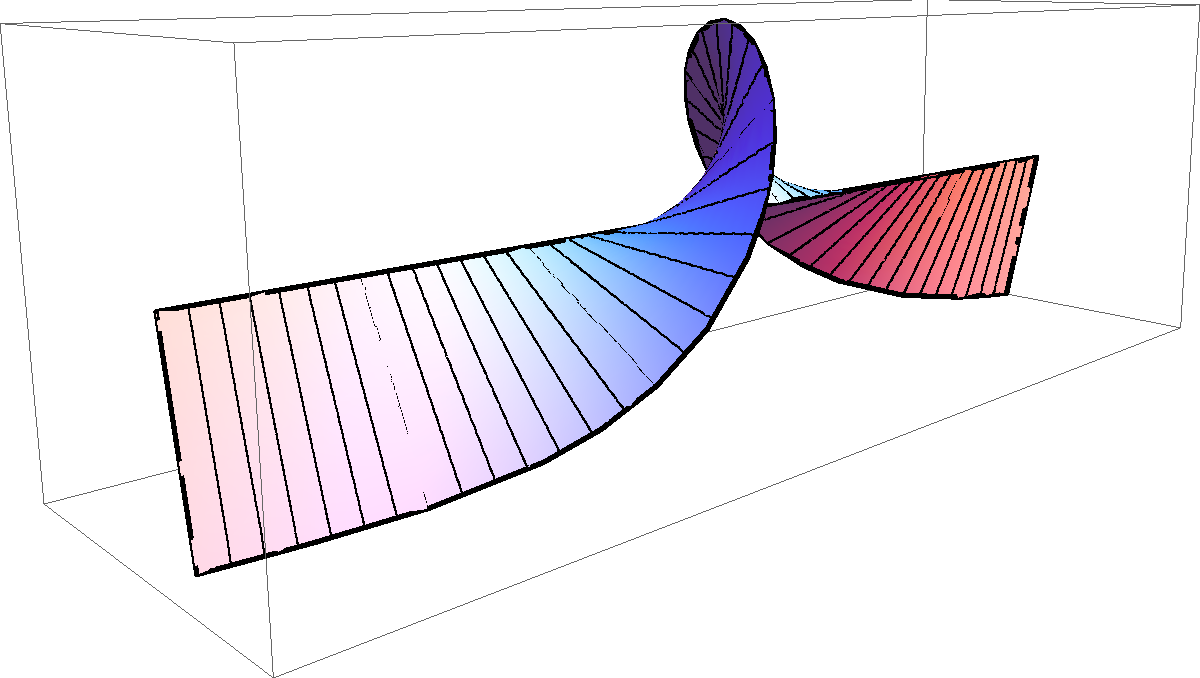
\includegraphics[width=0.5\linewidth,height=0.3\linewidth,clip]{./Bilder_SRT/Soliton_3D}
\caption[]{ \label{fig:Soliton}
Die Soliton-L\"osung: (oben links) Der Auslenkungswinkel $\varphi$ 
als Funktion der Koordinate $x$ entlang der Aufh\"angung,
(oben rechts) die Seitenansicht.}
% (unten) die dreidimensionale Ansicht.}
\end{figure}

Die Soliton-L\"osung entspricht einer Konfiguration, bei der sich die
Pendel in der N\"ahe eines Punktes einmal um ihre Aufh\"angung herumwinden, 
sich anderenfalls aber im Wesentlichen in der
senkrecht herabh\"angenden Ruhelage befinden (siehe Abb.\ \ref{fig:Soliton}). 
Diese L\"osung ist stabil. 
Die statische L\"{o}sung des Kontinuumsmodells ist durch
\index{Soliton}
\begin{equation}
\label{soliton}
      \varphi_0(x) ~=~ 4 \tan^{-1}
      \left( \exp \pm \sqrt{g}(x-x_0) \right) 
\end{equation}
gegeben, wobei die Integrationskonstante $x_0$ die Position
des Solitons angibt, d.h.\ den Punkt, bei dem $\varphi=\pi$. 
Das + Zeichen in (\ref{soliton}) entspricht einer L\"osung, f\"ur die
$\lim_{x\rightarrow -\infty} \varphi(x) \rightarrow 0$ und
$\lim_{x\rightarrow +\infty} \varphi(x) \rightarrow 2\pi$. Das $-$ 
Zeichen beschreibt eine so\-ge\-nann\-te Anti-Soliton-L\"osung mit
$\lim_{x\rightarrow -\infty} \varphi(x) \rightarrow 2\pi$ und
$\lim_{x\rightarrow +\infty} \varphi(x) \rightarrow 0$.
In beiden F\"allen n\"ahern sich die L\"osungen ihrem asymptotischen Wert
f\"ur gro\ss e $|x-x_0|$ exponentiell. Die Reichweite der L\"osung 
entspricht dabei
\begin{equation}
\label{width}
   \Delta L ~=~ 1/\sqrt{g}   \;.
\end{equation}
Diese Gr\"o\ss e ist ein Ma\ss\ f\"ur die halbe Breite des Solitons und
soll uns als L\"angenskala dienen. 

\begin{figure}[htbp]
\includegraphics[width=0.47\linewidth,height=0.28\linewidth,clip]{./Bilder_SRT/Breather_phi} \hspace{0.3cm}
\includegraphics[width=0.47\linewidth,height=0.28\linewidth,clip]{./Bilder_SRT/Breather_Height}%\\[0.5cm]
%\hspace*{3cm}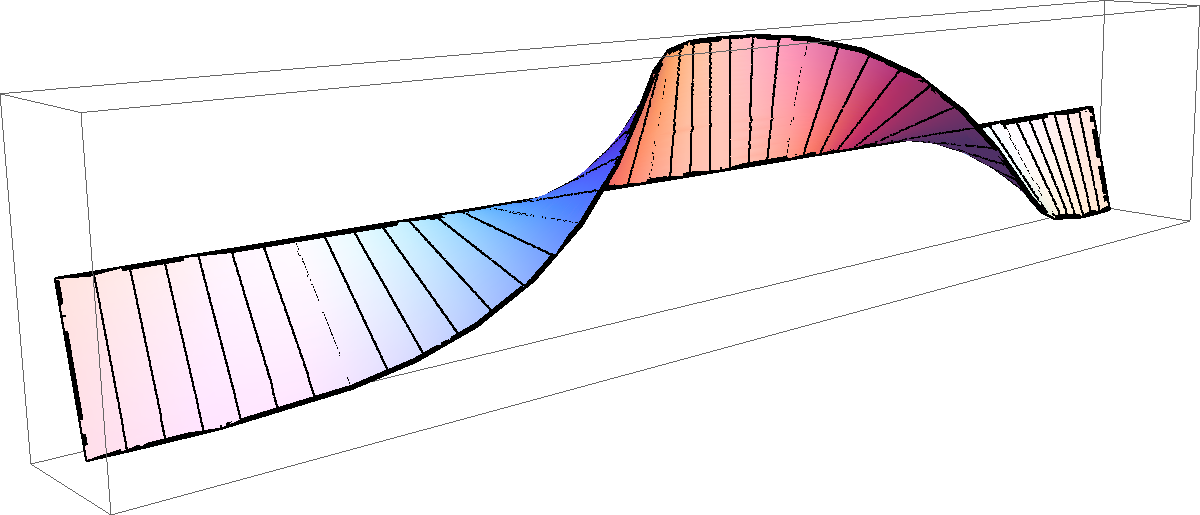
\includegraphics[width=0.5\linewidth,height=0.3\linewidth,clip]{./Bilder_SRT/Breather_3D}
\caption[]{ \label{fig:Breather}
Die Breather-L\"osung: (oben links) Der Auslenkungswinkel $\varphi$ 
als Funktion der Koordinate $x$ entlang der Aufh\"angung im
Augenblick maximaler Auslenkung,
(oben rechts) die Seitenansicht.}
%, (unten) die dreidimensionale Ansicht.}
\end{figure}

Die Sinus-Gordon Theorie besitzt ebenfalls L\"osungen, die gebundenen
Zust\"anden eines Solitons und eines Anti-Solitons entsprechen, die 
sogenannten Breather-L\"osungen (vgl.\ \cite{Lamb}; Darstellung in
Abb.\ \ref{fig:Breather}):
\index{Breather-L\"osung}
\begin{equation}
\label{breather}
    \varphi_0(x,t) ~=~ - 4 \tan^{-1} \left[ \frac{m}{\sqrt{1-m^2}}
    \frac{\sin \sqrt{g(1-m^2)}(t-t_0)}{\cosh m \sqrt{g}(x-x_0)} \right]\;.
\end{equation}
Der Parameter $m$ muss der Bedingung $0<m^2<1$ gen\"ugen, ist ansonsten 
aber beliebig. Die Schwingungsperiode ist
\begin{equation}
\label{time}
     \Delta T ~=~ \frac{2\pi}{\sqrt{g(1-m^2)}}~.
\end{equation}
Diese L\"osung ist metastabil. Es handelt sich um einen gebundenen
Zustand zwi\-schen einem Teilchen und seinem Antiteilchen, und kleine
St\"orungen lassen dieses System in \glqq Photonen\grqq\ zerfallen, d.h.\
einfache Schwingungen der Pendelkette. Der freie
Parameter $m$ h\"angt mit der Bindungsenergie zusammen und legt sowohl die
Amplitude als auch die Periode fest. Zur Festlegung einer Zeitskala
muss daher ein spezieller Wert f\"ur $m$ gew\"ahlt werden. Eine m\"ogliche
Wahl w\"are, dass $\varphi$ zwischen $-\pi$ und $+\pi$ variiert, d.h.\
$m^2=1/2$ oder $\Delta T=\sqrt{8\pi^2/g}$. (Dieser Wert f\"ur $m$ wurde
in Abb.\ \ref{fig:Breather} gew\"ahlt.)
\vspace{0.3cm}

Wir wollen nun untersuchen, wie sich die so definierten L\"angen-
und Zeitma\ss st\"abe transformieren, wenn man sie relativ zum
\glqq \"Ather\grqq, d.h.\ dem durch die Pendel definierten Ruhesystem,
bewegt.
Wir betrachten zun\"achst ein Soliton mit einer Geschwindigkeit
$v$. Diese L\"osung erhalten wir aus der statischen L\"osung nach 
Gleichung (\ref{eq_inv}). Auch die Breite des propagierenden Solitons
l\"asst sich daraus ablesen. 

Die statische L\"osung $\varphi_0(x)$ habe ihr Zentrum bei $x=0$. Dann
bestimmt die Bedingung
\[         \varphi_0(\pm \Delta L) ~=~ \pi \pm \alpha   \]
einen Wert f\"ur $\alpha$, bei dem wir die Breite von $\varphi_0$ messen.
F\"ur die propagierende L\"osung
\[         \varphi_v(x,t) ~=~ \varphi_0(\,\gamma(v)(x-vt)\,) \;,  \]
bewegt sich das Zentrum $x_0(t)$ nach der Gleichung $x_0(t)=vt$. Die
Breite dieser L\"osung ist gleich dem Wert $\Delta L_v$, der der
Bedingung
\[    \varphi_v(x_0(t)\pm \Delta L_v,t) ~=~ \pi \pm \alpha  \]
gen\"ugt. Dies ist offensichtlich der Fall f\"{u}r
\begin{equation}
\label{Lorentz}
        \gamma(v)\, \Delta L_v ~=~ \Delta L ~~~{\rm oder} ~~~
        \Delta L_v ~=~ \sqrt{1-v^2} \Delta L \;.  
\end{equation}
Die Breite der propagierenden L\"{o}sung ist daher um einen Faktor
$1/\gamma(v)$ kontrahiert. Diese \glqq Lorentz-Kontraktion\grqq\ kann von
\index{Lorentz-Fitzgerald-Kontraktion}
einem au\ss enstehenden Beobachter, der sieht, wie sich die Solitonen
entlang der Pendelkette ausbreiten, tats\"achlich wahrgenommen werden.

\begin{figure}[htbp]
\includegraphics[width=0.47\linewidth,height=0.28\linewidth,clip]{./Bilder_SRT/Soliton_Height} \hspace{0.3cm}
\includegraphics[width=0.47\linewidth,height=0.28\linewidth,clip]{./Bilder_SRT/Soliton_v09}
\begin{picture}(0,0)(0,0)
\thicklines
\put(-90,100){\vector(1,0){20}}
\put(-80,110){\makebox(0,0){$v=0{,}9$}}
\put(-280,110){\makebox(0,0){$v=0$}}
\end{picture}
\caption[]{ \label{fig:Soliton_v09}
Die Soliton-L\"osung in Bewegung: (links) Die ruhende 
Soliton-L\"osung aus Abb.\ \ref{fig:Soliton}, (rechts) 
die zugeh\"orige transformierte L\"osung zu einer 
Geschwindigkeit $v=0{,}9$.}
\end{figure}

Auch die Dilatation der Schwingungsperiode des gebundenen Zustands l\"asst
sich leicht herleiten. In Ruhe gilt f\"{u}r die Breather-L\"osung:
\[      \varphi_0^b(x,t) ~=~ \varphi_0^b(x,t+\Delta T) \;. \]
Die zugeh\"orige propagierende L\"osung erf\"ullt
\[   \varphi_v^b(x,t) ~=~ \varphi_v^b(x+v\Delta T_v, t+\Delta T_v) \;. \]
Da
\[   \varphi_v^b(x,t) ~=~
     \varphi_0^b \left(\,\gamma(v)(x-vt)\:,\:\gamma(v)(t-vx)\,\right)  \]
erhalten wir
\[   \gamma(v) \left( t+ \Delta T_v - v
     \left( x + v \Delta T_v \right) \right) ~=~
     \gamma(v) \left(t-v x \right) +
     \gamma(v) \left( 1-v^2\right) \Delta T_v \]
und somit:
\begin{equation}
\label{dilation}
      \Delta T ~=~ \gamma(v) \left(1-v^2 \right) \Delta T_v
      ~~~{\rm oder}~~~
      \Delta T_v ~=~ \frac{1}{\sqrt{1-v^2}} \Delta T \;.
\end{equation}
Die Schwingungsdauer eines sich bewegenden gebundenen Zustands ist
also tats\"achlich um einen Faktor $\gamma(v)$ im Vergleich zum ruhenden
Zustand verl\"angert.

Solitonen und gebundene Zust\"{a}nde von Solitonen k\"onnen an einem
festen Ende der Kette ohne Energieverlust reflektiert werden. Durch
eine solche experimentelle Anordnung kann man das 
\index{Zwillingsparadoxon}
\glqq Zwillingsparadoxon\grqq\ aufzeigen (vgl.\ Abschnitt \ref{chap_Zwilling}): 
Ein gebundener Zustand, der
sich entlang der Kette bewegt und nach einer Reflektion am Ende
der Kette zur\"uckkehrt, hat weniger Schwingungen ausgef\"uhrt, als ein
ruhender gebundener Zustand. Offensichtlich kann dieser Effekt
nicht der \glqq Beschleunigung\grqq\ am Ende der Kette
zugeschrieben werden.

\section{Von der \"Atherhypothese zur Relativit\"atstheorie}

Zun\"achst hat es vielleicht den Anschein, als ob das oben diskutierte
Modell der harmonisch gekoppelten Pendel sehr speziell sei. 
Hinsichtlich der Existenz von Soliton- und Breather-L\"osung mag das
richtig sein, nicht aber hinsichtlich der Tatsache, dass
dieses Modell den richtigen Verk\"urzungsfaktor und die richtige
Zeitdilatation liefert. Das einzige, was wir zur Herleitung dieser
Faktoren benutzt haben, ist die Lorentz-Invarianz der Feldgleichungen.
{\em Jede Lorentz-invariante Feldgleichung hat somit die Eigenschaft, dass
ihre L\"osungen, die eine L\"angen- oder Zeitskala definieren, sich genau
so transformieren, dass die bewegten Ma\ss st\"abe bzw.\ Uhren 
mit dem Lorentz'schen Verk\"urzungs- bzw.\ Dilatationsfaktor
multipliziert werden.}

Insbesondere haben auch die Maxwell-Gleichungen diese Eigenschaft.
Genau das hatte Lorentz gezeigt, wobei er allerdings noch die
falschen Transformationsgesetze f\"ur die Ladungen und Str\"ome
verwendet hatte. Diesen Fehler hat Poincar\'e korrigiert. Unter der 
Annahme, dass auf atomarer Ebene die 
Materie, und damit auch L\"angenma\ss st\"abe, durch die 
elektromagnetische Wechselwirkung zusammengehalten 
wird, war daher
die Lorentz-Kontraktion nicht nur plausibel sondern sogar eine
Folgerung aus den Maxwell-Gleichungen. 

Vor diesem Hintergrund k\"onnen wir auch den \"Ubergang
von der Lorentz'schen Sichtweise zur 
Einstein'schen Sichtweise und der 
speziellen Relativit\"atstheorie leichter nachvollziehen. 
Aus der Lorentz-Invarianz der fundamentalen Gleichungen
folgen ja nicht nur die Lorentz-Kontraktion und die Zeitdilatation,
sondern s\"amtliche Ph\"anomene, die sich im Rahmen der speziellen
Relativit\"atstheorie erkl\"aren lassen.

Oftmals wird behauptet, der \"Ubergang zur 
Sichtweise der speziellen Relativit\"atstheorie 
best\"unde in einer Neuinterpretation von 
\glqq Raum\grqq\ und \glqq Zeit\grqq.
Doch \"uber Raum und Zeit als abstrakte Entit\"aten 
k\"onnen wir eigentlich nichts sagen. In der Physik
interessieren wir uns nur f\"ur r\"aumliche und zeitliche
{\em Distanzen}, und diese Distanzen messen wir mir
physikalischen Instrumenten -- L\"angenma\ss st\"aben
und Uhren --, die selbst den physikalischen Gesetzen
unterliegen. 

Bisher bezog sich das Symbol $x$ auf 
eine Koordinate im Ruhesystem des
\"Athers -- im obigen Modell war dies das 
Ruhesystem der Pendelaufh\"angung. 
Dies entspricht dem \glqq Lineal\grqq\ eines 
externen Beobachters, der au\ss erhalb
unserer Welt steht und alles mit 
seinen Ma\ss st\"aben ausmessen kann -- 
wie wir bei den gekoppelten Pendeln. Entsprechend 
bezog sich auch das Symbol $t$ auf die Uhr eines externen Beobachters. Wir als
externe Beobachter k\"onnen die L\"angenkontraktion der Solitonen 
nachweisen, indem wir einfach ein \glqq externes\grqq\ 
Lineal neben das Soliton halten. Ebenso 
k\"onnen wir den propagierenden gebundenen Zustand beobachten und die 
Dilatation in der Schwingungsperiode 
mit unserer externen Uhr vergleichen. F\"ur uns als externe
Beobachter sind Raum (gemessen entlang der Pendelkette) und Zeit absolut. 
$c=1$ (die Geschwindigkeit von Wellen bzw.\ kleinen St\"orungen entlang der
Kette) ist f\"ur uns keine obere Grenzgeschwindigkeit, und wenn wir uns
entlang der Kette bewegen, ist die Ausbreitungsgeschwindigkeit einer
St\"orung entlang der Kette (das entspricht der Ausbreitung des Lichts)
in unserem System f\"{u}r die Vorw\"arts- und
R\"uckw\"artsrichtung verschieden: Das Ruhesystem der Pendelkette ist ein
ausgezeichnetes System.

Stellen wir uns nun jedoch (1+1)-dimensionale Wesen vor, die in dieser
\glqq Soliton-Welt\grqq\ leben. Ihnen stehen nur die Solitonen bzw.\ andere 
L\"osungen ihrer \glqq universellen Be\-we\-gungs\-glei\-chungen\grqq\ 
als L\"angen- und Zeitma\ss st\"abe zur Verf\"{u}gung. Sie werden daher
die Breite eines Solitons und die Schwingungsdauer der Breather-L\"osung
als L\"angen- und Zeitma\ss stab zur Beschreibung der physikalischen
Ph\"anomene benutzen. Doch wenn sie ein bewegtes Soliton mit
der Breite eines anderen bewegten Solitions vergleichen, \glqq messen\grqq\
sie keine Verk\"urzung, entsprechend messen sie auch mit
bewegten Breather-L\"osungen keine Ver\"anderungen in der
Zeitskala eines entsprechend bewegten Systems. Erst wenn sie
die Breite oder Zeitskalen von bewegten Systemen mit denen
von anders bewegten oder ruhenden Systemen vergleichen,
messen sie Unterschiede.

Der \"Ubergang zur Minkowski-Welt erfolgt gerade 
dadurch, dass die externen L\"angen- und Zeitma\ss st\"abe 
durch interne L\"angen- und Zeitma\ss st\"abe, die
denselben physikalischen Gesetzen unterliegen,
ersetzt werden. Es ist der \"Ubergang von
einer externen zu einer internen Perspektive.
Die zugrundeliegende diskrete Struktur 
und damit das ausgezeichnete Ruhesystem (der \glqq \"Ather\grqq) zeigen sich 
erst, wenn $v$ so gro\ss\ wird, dass die Brei\-te der Solitonen mit der 
Gr\"o\ss enordnung des 
Pendelabstands (bzw.\ der Gitterstruktur) vergleichbar wird. Ist die
fundamentale Theorie eine Kontinuumstheorie, 
so tritt der \glqq \"Ather\grqq\ 
f\"ur einen internen Beobachter \"uberhaupt nicht in Erscheinung.

Wenn wir von der Lorentz-Invarianz bzw.\ allgemeiner Poincar\'e-Invarianz
\index{Lorentz-Invarianz}
der Raum-Zeit sprechen, sollten wir eigentlich zwei Schritte bzw.\
Aspekte unterscheiden. Wir haben oben die Invarianzeigenschaft der
Bewegungsgleichungen als eine Eigenschaft der L\"osungsmenge dieser
Gleichungen interpretiert: Mit jeder L\"osung
$\varphi(x)$ ist auch $\varphi^{(\Lambda,a)}(x)=\varphi(\Lambda x -a)$  
eine L\"osung der Bewegungsgleichung. Gibt es nun ausgezeichnete
L\"osungen, die L\"angenma\ss st\"abe oder Uhren definieren, so bedeutet
diese Invarianz, dass bewegte L\"angenma\ss st\"abe k\"urzer, bewegte
Uhren langsamer erscheinen. Dies gilt zun\"achst bez\"uglich der
festen \glqq Hintergrunds-Raum-Zeit\grqq. Diesen Schritt hatte auch Lorentz
erkannt. Der wesentliche zweite Schritt aber blieb Einstein vorbehalten.
Er erkannte n\"amlich, dass die Poincar\'e-Invarianz einer Gleichung
auch bedeutet, dass bez\"uglich der intrinsischen Ma\ss st\"abe
das Relativit\"atsprinzip gilt und damit kein Inertialsystem
mehr ausgezeichnet ist. 

Statt die Lorentz-Invarianz der Gleichungen als Eigenschaft der
L\"osungsmenge anzusehen, was beispielsweise auch f\"ur die diskretisierte
Pendelkette einfach zu interpretieren war, k\"onnen wir die 
Lorentz-Invarianz auch als eine Freiheit der Koordinatenwahl auffassen.
Wenn wir n\"amlich die Raum- und Zeitkoordinaten einer 
Lorentz-Transformation unterwerfen, f\"ur eine Raumdimension somit
die Ersetzung
\begin{equation}
\label{LT}
   x \rightarrow x' ~=~ \frac{x - vt}{\sqrt{1-\beta^2}}  
    \hspace{0.5cm} {\rm und} ~~
    t \rightarrow t' ~=~ \frac{t - \frac{v}{c^2}x}{\sqrt{1-\beta^2}}
    \hspace{1cm} \left(\beta = \frac{v}{c} \right)  
\end{equation}    
vornehmen,
dann bleiben die Feldgleichungen unver\"andert. Ordnen wir nun die
Koordinaten $(x,t)$ bzw.\ $(x',t')$ jeweils Beobachtern zu, deren Weltlinie 
durch $x=0$ bzw.\ $x'=0$ und deren 
\glqq gleichzeitige Ereignisse\grqq\ 
durch die Bedingungen $t=$const.\ bzw.\ $t'=$const.\ definiert sind,
dann bedeutet die Invarianz der Feldgleichungen, dass beide Beobachter
dieselbe Physik sehen, d.h., es gilt das Relativit\"atsprinzip.  

Die Lorentz-Invarianz der Bewegungsgleichungen k\"onnen wir
offensichtlich physikalisch auf zwei vollkommen unterschiedliche Weisen
interpretieren. Einmal als Eigenschaft der L\"osungsmenge, die es uns
erlaubt, aus bestimmten L\"osungen andere zu gewinnen. Diese 
Interpretation bezieht alles auf einen festen Satz von Koordinaten $(x,t)$
(vgl.~(\ref{eq_inv})), der als das Koordinatensystem eines ausgezeichneten
Ruhesystems interpretiert werden kann. Bez\"uglich dieser Koordinaten
beobachten wir die Lorentz-Kontraktion und die Zeitdilatation. 

Die andere Interpretation impliziert das Relativit\"atsprinzip. Wenn
sich zwei Beobachter relativ zueinander mit einer konstanten 
Geschwindigkeit $v$ bewegen, k\"onnen sie unterschiedliche
Koordinatensysteme verwenden, in denen sie sich jeweils im
Ursprung (und damit in Ruhe) befinden. Jeder verwendet zur
Angabe von r\"aumlichen und zeitlichen Distanzen Werte, die mit 
Instrumenten in seinem System gemessen wurden. 
Die von den beiden Beobachtern verwendeten 
Koordinaten h\"angen \"uber die Gleichungen
(\ref{LT}) miteinander zusammen. In diesem Fall erfahren beide
Beobachter dieselbe Physik. In dieser Interpretation gibt es kein
ausgezeichnetes Ruhesystem -- der \"Ather ist verschwunden. 
Der Preis ist eine neue Vorstellung von Gleichzeitigkeit. Dieser letzte
Schritt zeichnete Einstein vor Lorentz und Poincar\'e aus. 
      
\section{Die Synchronisation von Uhren}
\label{sec_Synch}

Ein ungewohnter (und in manchen Kreisen immer noch umstrittener) Aspekt der speziellen
Relativit\"atstheorie ist ihr Konzept von Gleichzeitigkeit. 
Dabei wird\index{Gleichzeitigkeit}
oft vergessen, dass es sich bei der Behauptung, zwei 
Ereignisse seien gleichzeitig, nicht um eine
\glqq faktische\grqq\ Aussagen handelt, sondern 
eher um eine Konvention.\footnote{Versteht man unter \glqq faktisch\grqq, dass
sich alle Beobachter unabhh\"angig von ihrem Bezugssystem in einer Aussage
einig sind, so ist die Gleichzeitigkeit in der Newton'schen Physik faktisch, in der
Relativit\"atstheorie jedoch nicht.}
Ob zwei Ereignisse f\"ur ein gegebenes Inertialsys\-tem gleichzeitig
stattfinden oder
nicht, k\"onnen wir experimentell nur entscheiden, wenn wir eine
Vorschrift angeben, was wir unter \glqq gleichzeitig\grqq\ verstehen
wollen. Diese Vorschrift wird letztendlich darin bestehen, dass wir
zwei Ereignisse als gleichzeitig ansehen, wenn die Uhren
am jeweiligen Ort dieser Ereignisse dieselbe Zeit anzeigen, womit wir das
Problem auf die Synchronisation von Uhren an verschiedenen
Orten (aber im selben Inertialsystem) reduzieren haben. 
Die einzige Einschr\"ankung ist, dass zwei gleichzeitige 
Ereignisse $A$ und $B$ {\em nicht} in einer kausalen Abh\"angigkeit stehen 
sollten. Grunds\"atzlich k\"onnen wir
eine beliebige raumartige Hyperfl\"ache als gleichzeitig {\em definieren}.

Die folgenden \"Uberlegungen gelten f\"ur den flachen Minkowski-Raum.
Wir konzentrieren uns ausschlie\ss lich auf den Aspekt der
Synchronisation\index{Synchronisation von Uhren} 
von Uhren f\"ur ein gegebenes Inertialsystem. Eine
ausf\"uhrlichere Darstellung dieser Problematik findet man bei 
Mittelstaedt \cite{Mittelstaedt} sowie in den beiden Abhandlungen
{\em Philosophie der Raum-Zeit-Lehre} \cite{Reichenbach1} und 
{\em Axiomatik der relativistischen Raum-Zeit-Lehre} \cite{Reichenbach2}
von Hans Reichenbach\index{Reichenbach, Hans} 
(Hans Friedrich Herbert G\"unther Reichenbach,
{\em geb.\ 26.9.1891 in Hamburg; gest.\ 9.4.1953 in Los Angeles}). 

\subsection{Synchronisation durch Lichtsignale}

Zun\"achst ist es recht hilfreich, sich bei der operationalen
Definition von Gleichzeitigkeit auf ein 
allgemeines Verfahren zu beschr\"anken, das allerdings
noch keine Einschr\"ankung an die M\"oglichkeiten darstellt. 
Wir wollen Uhren durch
Austausch von Lichtsignalen synchronisieren. Beobachter $A$ sendet zum
Zeitpunkt $t_1$ ein Lichtsignal aus. Dieses wird von Beobachter $B$
reflektiert und erreicht Beobachter $A$ zum Zeitpunkt $t_2$. Bezeichnen
wir den Zeitpunkt des Ereignisses der Reflektion des Lichtstrahls bei
Beobachter $B$ mit $t$, so m\"ochte Beobachter
$A$ nun definieren, welches Ereignis auf seiner Weltlinie zu
dem Moment der Reflektion des Lichtstrahls bei Beobachter $B$ gleichzeitig
war, d.h.\ dem Zeitpunkt $t$ entspricht. Die einzige Einschr\"ankung
liefert dabei die Forderung der Kausalit\"at: $t_1 < t < t_2$. Beobachter
$A$ definiert nun:
\[      t ~=~ t_1 + \epsilon(A,B) (t_2 - t_1)     \]
mit 
\[         0 < \epsilon(A,B) < 1  \;.   \]
(Der Einfachheit halber soll das Synchronisierungsverfahren nicht von
der Zeit abh\"angen, d.h.\ $\epsilon(A,B)$ h\"angt nicht zus\"atzlich
noch von $t$ bzw.\ $t_1$ ab.)   

\begin{SCfigure}[50][htb]
\begin{picture}(120,200)(0,0)
\put(20,20){\line(0,1){180}}
\put(80,20){\line(0,1){180}}
\put(20,50){\line(1,1){60}}
\put(20,170){\line(1,-1){60}}
\put(20,80){\line(2,1){60}}
\put(20,10){\makebox{$A$}}
\put(80,10){\makebox{$B$}}
\put(50,0){\makebox{(a)}}
\put(10,50){\makebox{$t_1$}}
\put(10,170){\makebox{$t_2$}}
\put(6,78){\makebox{$x_A$}}
\put(84,108){\makebox{$x_B$}}
\end{picture}
%
\begin{picture}(100,200)(0,0)
\put(20,20){\line(0,1){180}}
\put(80,20){\line(0,1){180}}
\put(20,70){\line(1,1){60}}
\put(20,190){\line(1,-1){60}}
\put(20,100){\line(2,1){60}}
\put(20,100){\line(1,1){60}}
\put(20,100){\line(1,-1){60}}
\put(20,10){\makebox{$A$}}
\put(80,10){\makebox{$B$}}
\put(50,0){\makebox{(b)}}
\put(10,70){\makebox{$t_1$}}
\put(10,190){\makebox{$t_2$}}
\put(7,98){\makebox{$x_A$}}
\put(84,128){\makebox{$x_B$}}
\put(84,40){\makebox{$t'_1$}}
\put(84,160){\makebox{$t'_2$}}
\end{picture}
\caption{\label{figsyn}%
Synchronisation von Uhren durch Lichtstrahlen. Die senkrechten Linien
entsprechen den Weltlinien der Beobachter $A$ und $B$, die zueinander
einen konstanten Abstand halten. (a) Zum Zeitpunkt $t_1$ sendet $A$ ein
Lichtsignal aus, das von $B$ im Ereignis $x_B$ reflektiert wird und
bei $t_2$ wieder Beobachter $A$ erreicht. Durch Vorgabe von $\epsilon_A$
konstruiert $A$ das Ereignis $x_A$, das zu $x_B$ gleichzeitig ist.
(b) Soll die Gleichzeitigkeit der Ereignisse $x_A$ und $x_B$ auch f\"ur
Beobachter $B$ gelten, so muss er sein Verfahren zur Bestimmung der
Gleichzeitigkeit (ausgedr\"uckt durch $\epsilon_B$) so w\"ahlen, 
dass $\epsilon_B=1-\epsilon_A$.} 
\end{SCfigure}

Zun\"achst kann man sich leicht \"uberzeugen, dass durch geeignete 
Wahl von $\epsilon$ tats\"achlich je zwei raumartige Ereignisse $x_A$ und
$x_B$ auf der Weltlinie von $A$ und $B$ als gleichzeitig 
definiert werden k\"onnen (vgl.\ Abb.~\ref{figsyn}). 
Dieses Verfahren bildet daher keine Einschr\"ankung der Allgemeinheit. 
Damit die Hyperfl\"ache der zu $x_A$ gleichzeitigen Ereignisse eine
raumartige Hyperfl\"ache ist, m\"ussen die Richtungsableitungen der 
Funktion $\epsilon(A,B)$ (aufgefasst als eine Funktion von $B$) noch
durch eine Konstante (bei unserer Definition der Lichtgeschwindigkeit
ist diese Konstante 1) beschr\"ankt sein. Durch geeignete Forderungen
an die Funktion $\epsilon$ erh\"alt man verschiedene 
Synchronisationsverfahren.

\subsection{Die Einstein-Synchronisation}

Eine sehr allgemeine Forderung an die Gleichzeitigkeit von Ereignissen
\index{Symmetrie der Gleichzeitigkeit}
ist die Symmetrieforderung: Wenn f\"ur einen Beobachter $A$ das 
Ereignis $x_B$ auf der Weltlinie eines Beobachters $B$ gleichzeitig zu
dem Ereignis $x_A$ auf seiner Weltlinie ist, dann soll umgekehrt auch
f\"ur den Beobachter $B$ das Ereignis $x_A$ gleichzeitig zu $x_B$ sein.
Anhand der Abbildung \ref{figsyn}(b) kann man sich leicht \"uberzeugen,
dass diese Forderung gleichbedeutend mit der Bedingung
\[          \epsilon(A,B) ~=~ 1 - \epsilon(B,A)      \]
ist. 

Eine weitere allgemeine Forderung ergibt sich aus der Homogenit\"at des
\index{Homogenit\"at des Raumes}
Raumes. Wir verlangen, dass sich die Funktion $\epsilon(A,B)$ nicht
\"andert, wenn wir die beiden Beobachter $A$ und $B$ um {\em denselben}
(r\"aumlichen) Vektor verschieben. Symbolisch ausgedr\"uckt:
\[     \epsilon(A+\vec{a},B+\vec{a}) ~=~ \epsilon(A,B)     \;.  \]
Dies bedeutet, dass $\epsilon(A,B)$ nur noch von der r\"aumlichen 
Richtung abh\"angen kann, unter der der Beobachter $B$ von $A$ aus gesehen
wird. Innerhalb einer Halbebene, die die Weltlinie von $A$
als Rand hat, ist $\epsilon$ konstant. Auch diese Forderung verlangen
wir allgemein.

Nun kommen wir zu einer speziellen Forderung, die sich aus der Konstanz
der Lichtgeschwindigkeit ergibt. Da die Lichtgeschwindigkeit f\"ur jeden
Beobachter und f\"ur jede Richtung dieselbe sein soll, k\"onnen wir
zus\"atzlich noch Isotropie 
\index{Isotropie des Raumes}
unserer Gleichzeitigkeitsdefinition verlangen.
$\epsilon$ soll also auch nicht mehr von der r\"aumlichen Richtung 
abh\"angen, unter der $B$ von $A$ aus gesehen wird. In diesem Fall 
gilt
\[       \epsilon(A,B) ~=~ {\rm const}    \;.  \]
Zusammen mit der ersten Forderung der Symmetrie folgt sofort:
\[       \epsilon ~=~ \frac{1}{2}  \;.   \]
Die aus diesem Wert f\"ur $\epsilon$ folgende Synchronisation von
Uhren bezeichnet man als\index{Einstein-Synchronisation} 
Einstein-Synchronisation. 

Das zweite Axiom der speziellen Relativit\"atstheorie - die Konstanz
der Lichtgeschwindigkeit - f\"uhrt uns somit schon zur Festlegung der
Gleichzeitigkeitsvorschrift. Das erste Axiom - 
das Relativit\"atsprinzip\index{Relativit\"atsprinzip} -
geht indirekt in diese Festlegung ein, da wir die Konstanz der 
Lichtgeschwindigkeit und somit die Isotropie der
Synchronisationsvorschrift f\"ur jedes Inertialsystem verlangt haben. 
  
\subsection{Synchronisation mit der \"Atherhypothese}

Wir haben aus der Lorentz-Invarianz der universellen Bewegungsgleichungen
geschlossen, dass die spezielle Relativit\"atstheorie in der 
Formulierung von Einstein \"aquivalent zur Lorentz-Theorie ist, d.h.\
zu einer Theorie mit \"Atherhypothese und Lorentz-Kon\-traktion der
L\"angenskalen. Es sollte daher nicht \"uberraschen, wenn es eine
Synchronisationsvorschrift gibt, die auf die Lorentz-Theorie f\"uhrt.

\begin{figure}[ht]
\begin{picture}(360,200)(0,0)
\put(30,120){\vector(1,0){120}}
\put(80,10){\vector(0,1){170}}
\put(30,20){\line(1,2){80}}
\thicklines
\put(40,40){\line(1,1){80}}
\put(120,120){\line(-1,1){27}}
\thinlines
\put(80,120){\makebox(0,0){{\footnotesize $\bullet$}}}
\put(120,120){\makebox(0,0){{\footnotesize $\bullet$}}}
\put(40,40){\makebox(0,0){{\footnotesize $\bullet$}}}
\put(93,147){\makebox(0,0){{\footnotesize $\bullet$}}}
\put(75,125){\makebox(0,0){$O$}}
\put(32,40){\makebox(0,0){$A$}}
\put(87,150){\makebox(0,0){$B$}}
\put(123,128){\makebox(0,0){$C$}}
\put(75,180){\makebox(0,0){$t$}}
\put(150,115){\makebox(0,0){$x$}}
\put(100,10){\makebox(0,0){(a)}}
%
\put(210,120){\vector(1,0){120}}
\put(260,10){\vector(0,1){170}}
\put(210,20){\line(1,2){80}}
\put(220,80){\line(2,1){100}}
\thicklines
\put(220,40){\line(1,1){80}}
\put(300,120){\line(-1,1){27}}
\thinlines
\put(246.5,93){\makebox(0,0){{\footnotesize $\bullet$}}}
\put(300,120){\makebox(0,0){{\footnotesize $\bullet$}}}
\put(220,40){\makebox(0,0){{\footnotesize $\bullet$}}}
\put(273,147){\makebox(0,0){{\footnotesize $\bullet$}}}
\put(255,125){\makebox(0,0){$O$}}
\put(212,40){\makebox(0,0){$A$}}
\put(267,150){\makebox(0,0){$B$}}
\put(303,128){\makebox(0,0){$C$}}
\put(240,97){\makebox(0,0){$D$}}
\put(255,180){\makebox(0,0){$t$}}
\put(330,115){\makebox(0,0){$x$}}
\put(280,10){\makebox(0,0){(b)}}
\end{picture}
\caption{\label{figuhr}%
\"Ather- und Einstein-Synchronisation. In Teil (a) rekonstruiert der
Beobachter auf der Weltlinie $AB$ das Ereignis $O$ als gleichzeitig zum
Ereignis $C$. Seine Synchronisationsvorschrift h\"angt von der 
Geschwindigkeit $v$ relativ zu dem ausgezeichneteten Ruhesystem ab.
Dabei gilt f\"ur das Verh\"altnis $(AO)/(AB)=(1+v)/2$. 
In Abbildung (b) wird nach der Einstein-Synchronisation aus denselben
Lichtsignalen das Ereignis $D$ als zu $C$ gleichzeitig rekonstruiert.}
\end{figure}

Auch mit \"Atherhypothese verlangen wir von der Gleichzeitigkeit von
\index{Aetherhypothese@\"Atherhypothese}
Ereignissen Symmetrie und Homogenit\"at des Raumes. Was wir jedoch
nicht mehr verlangen k\"onnen, ist die allgemein g\"ultige Isotropie
der Synchronisationsvorschrift. F\"ur ein System, das sich relativ zum
\"Ather mit einer Geschwindigkeit $\vec{v}$ bewegt, wird die
Synchronisationsvorschrift von der Richtung relativ zu $\vec{v}$
abh\"angen. Allgemein wird also nun gelten:
\[         \epsilon(A,B) ~=~ \epsilon(\vec{v};A,B)   \;.   \]
Lediglich f\"ur das ausgezeichnete Inertialsystem, das dem
Ruhesystem des \"Athers entspricht, ist die Lichtgeschwindigkeit in
alle Richtungen dieselbe und somit das Synchronisationsverfahren
symmetrisch:
\[       \epsilon(\vec{v}=0;A,B) ~=~ \frac{1}{2}   \;.   \]
Bewegt sich das Inertialsystem der Beobachter $A$ und $B$ relativ
zum \"Ather mit der Geschwindigkeit $\vec{v}$, so gilt 
(vgl.\ Abb.~\ref{figuhr})
\[      \epsilon(\vec{v};A,B) ~=~ \frac{1}{2} 
        \left( 1 + \frac{|\vec{v}|}{c}\cos \alpha \right)  \;, \]
wobei $\alpha$ der Relativwinkel zwischen der Richtung von $\vec{v}$
und der Halbebene ist, die durch die Weltlinie
von $A$ begrenzt wird und die Weltlinie von $B$ enth\"alt.

Der Vorteil dieses Verfahrens ist, dass Gleichzeitigkeit nun
ein absoluter Begriff wird. Sind zwei Ereignisse $x_A$ und $x_B$
f\"ur einen Beobachter $A$ gleichzeitig, so sind sie es auch f\"ur
alle anderen Beobachter, unabh\"angig von deren Bewegungszustand.
 
Der Nachteil dieses Verfahrens ist jedoch, dass wir das Ruhesystem
des \"Athers nicht kennen. Wir m\"ussen also willk\"urlich ein System
auszeichnen, das wir als Ruhesys\-tem definieren, beispielsweise das
System des Schwerpunkts der in unserem Universum beobachtbaren Massen
oder das Ruhe\-sys\-tem relativ zur Hintergrundstrahlung. (Es ist nicht
selbstverst\"andlich, dass diese beiden Sys\-teme identisch sind.)
Wegen der Geschwindigkeitsabh\"angigkeit des Synchronisationsverfahrens
gilt das Relativit\"atsprinzip nicht mehr. Die Lichtgeschwindigkeit
ist nur im Ruhesystem des \"Athers richtungs\-un\-ab\-h\"angig konstant.

Das Relativit\"atsprinzip gilt jedoch in einer anderen Form:
Wir k\"onnen jedes beliebige Inertialsystem als Ruhesystem definieren
und die Synchronisation der Uhren auf dieses System beziehen. Die
physikalischen Gesetze bleiben dieselben. Hier liegt der physikalisch
unbefriedigende Aspekt dieses Synchronisierungsverfahrens. Wir brechen
die Symmetrie, die sich im Relativit\"atsprinzip ausdr\"uckt,
{\em per Hand}, indem wir ein Inertialsystem auszeichnen. Umgekehrt
tr\"agt die Einstein-Synchronisation dem Relativit\"atsprinzip Rechnung.
Kein Inertialsystem wird durch dieses Verfahren ausgezeichnet. Der
Preis ist allerdings die Relativit\"at der Gleichzeitigkeit.

Unter bestimmten Unst\"anden ist es jedoch sinnvoll, eine
Synchronisation zu w\"ahlen, die der Lorentz'schen Sichtweise
n\"aher ist als der Einstein'schen. Beispielsweise k\"onnte man
die Lorentz'sche Sichtweise so interpretieren, dass iregendwo in der Mitte
unseres Universums eine riesige Uhr steht, und das, was diese Uhr anzeigt,
ist die \glqq wahre\grqq\ Zeit. Alle anderen Systeme m\"ussen ihre Zeit auf
diese wahre Zeit umrechnen. Dieses Verfahren wird in abgewandelter Form
beispielsweise bei der Zeitsynchronisation des GPS-Satellitensystems verwendet.
Die \glqq riesige Uhr\grqq\ steht in der GPS-Zentrale in Colorado. Die 
Uhren der Satelliten sind so geschaltet, dass ihre Zeit gleich der 
\glqq Masterzeit\grqq\ ist. Insbesondere ist ihr Gang im 
Vergleich zu einer \glqq richtigen\grqq\
Uhr etwas gedrosselt, um den Einfluss der schw\"acheren Gravitation sowie
der Bewegung auszugleichen.

Die Einstein-Synchronisation wie auch die 
\glqq \"Athersynchronisation\grqq\
sind Spezialf\"alle einer Klasse von Synchronisationsvorschriften, bei
denen die Konstanz der sogenannten \glqq Zwei-Wege-Lichtgeschwindigkeit\grqq\
\index{Zwei-Wege-Lichtgeschwindigkeit}%
gefordert wird. Dabei handelt es sich um die Geschwindigkeit $c$, die
man einem Lichtstrahl zuordnet, der eine Strecke in beide Richtungen -
vor und zur\"uck - durchl\"auft. Ist $c^+$ die Geschwindigkeit f\"ur
eine Richtung und $c^-$ die Geschwindigkeit f\"ur die R\"uckrichtung,
so ist
\[   \frac{1}{c} ~=~ \frac{1}{2} \left( \frac{1}{c^+} + \frac{1}{c^-}
                  \right)   \;.    \]
W\"ahrend jedoch zur Messung von $c^+$ bzw.\ $c^-$ die Uhren an 
verschiedenen
Raumpunkten synchronisiert sein m\"ussen, kann man $c$ an einem Punkt
auswerten, d.h.\ $c$ h\"angt nicht von der Synchronisationsvorschrift
ab. Im Michelson-Morley-Versuch\index{Michelson-Morley-Experiment} 
beispielsweise wird die Lichtgeschwindigkeit
ja gar nicht f\"ur verschiedenen Raumrichtungen verglichen, sondern nur
die Zwei-Wege-Lichtgeschwindigkeit. Nur von dieser wird gezeigt, dass
sie isotrop ist. Die Einstein'sche Forderung der Konstanz der
Lichtgeschwindigkeit geht also \"uber das Ergebnis des 
Michelson-Morley-Versuchs hinaus.

\subsection{Synchronisation durch langsamen Uhrentransport} 

Abschlie\ss end soll noch gezeigt werden, dass die
Synchronisation durch langsamen Uhrentransport zu demselben
Ergebnis wie die Einstein-Synchronisation f\"uhrt. 
Das bedeutet Folgendes: Synchronisiert man zwei Uhren am selben Ort
und bringt dann die eine der beiden Uhren
langsam zu einem anderen Ort, ist die so
erreichte Synchronisation eine Einstein-Synchronisation.

Zun\"achst sollten wir etwas genauer definieren,
was \glqq Synchronisation durch langsamen Uhrentransport\grqq\
bedeutet. Wir stellen uns dazu zwei Beobachter vor, die
einen konstanten Abstand $L$ halten und sich im
selben Inertialsystem befinden. Zu einem Zeitpunkt $t_0=0$ werden bei
Beobachter 1 zwei Uhren synchronisiert. Anschlie\ss end
wird eine der beiden Uhren mit der Geschwindigkeit $v$
zu Beobachter 2 gebracht. Sie ben\"otigt dazu f\"ur 
Beobachter 1 die Zeit $t=L/v$, das ist also die Zeit,
die Beobachter 1 dem Ereignis \glqq Uhr ist bei Beobachter 
2\grqq\ zuschreiben wird. Die Anzeige auf
der Uhr ist allerdings nach der Relativit\"atstheorie etwas k\"urzer, n\"amlich
\begin{equation}
\label{eq_Korrektur}
           t_1 = \sqrt{1-\frac{v^2}{c^2}} t \, .  
\end{equation}
Wir k\"onnen nicht einfach argumentieren, dass
f\"ur $v/c\ll 1$ die rechte Seite gegen $t$ geht,
denn wenn $v$ sehr klein ist, wird $t$ sehr gro\ss,
und damit  w\"urde zwar $t_1/t$ gegen 1 gehen,
aber $t_1$ und $t$ k\"onnten sich m\"oglicherweise
selbst im Limes $v\rightarrow 0$ noch um einen konstanten
Term unterscheiden. Es gilt aber
\begin{equation}
       t_1 = \left( 1 - \frac{v^2}{c^2} + O((v/c)^4) \right) \frac{L}{v}
       \approx \frac{L}{v} - \frac{L}{c}\frac{v}{c} + ... 
       = t -  \frac{L}{c}\frac{v}{c} + ...
\end{equation} 
Da $L$ und $c$ Konstanten sind ($L/c$ ist die Zeit, die das
Licht braucht, die Strecke $L$ zu durchqueren), wird
der Korrekturterm f\"ur sehr kleine Geschwindigkeiten
beliebig klein. Allerdings ist die Korrektur von der
Ordnung $v/c$ und nicht, wie man zun\"achst nach
Gleichung \ref{eq_Korrektur} erwarten k\"onnte,
von der Ordnung $(v/c)^2$. 
 
\begin{thebibliography}{99}
\addcontentsline{toc}{chapter}{Literaturangaben}
\bibitem{Lamb} G.L.\ Lamb, Jr.; {\it Elements of Soliton Theory}; 
         Pure \& Applied Mathematics, John Wiley \& Sons, 1980. 
\bibitem{Mittelstaedt} Peter Mittelstaedt; {\it Der Zeitbegriff in der
        Physik}; BI-Wissenschaftsverlag, 1989.        
\bibitem{Reichenbach1} Hans Reichenbach; {\em Philosophie der 
       Raum-Zeit-Lehre}; Hans Reichenbach - Gesammelte Werke Bd.\ 2;
       Vieweg-Verlag, Braunschweig; 1977.
\bibitem{Reichenbach2} Hans Reichenbach; {\em Axiomatik der
       relativistischen Raum-Zeit-Lehre}; in {\em Die philosophische
       Bedeutung der Relativit\"atstheorie}; Hans Reichenbach - Gesammelte
       Werke Bd.\ 3; Vieweg-Verlag, Braunschweig, 1977. 
\end{thebibliography}
  
\end{document}
